% Chapter Template

\chapter{存储分离} % Main chapter title

\label{Chapter3} % Change X to a consecutive number; for referencing this chapter elsewhere, use \ref{ChapterX}

存储设备是用于存储信息的设备,也被称为外存。
相比于内存,它容量大、廉价,但是读写速度慢。
与内存相似,单台服务器上面能接入的存储设备数量也是有限的。

然而,无论是容量还是读写速度,应用程序对硬盘资源的需求还是十分巨大的,如何用一种有效的组织方式来管理和使用硬盘资源是数据中心里面的焦点问题。
存储分离(storage disaggregation)也是其中一个重要的研究方向。
与内存分离的定义相似,存储分离技术让应用程序同时能够访问本地服务器和远端服务器的存储设备,将存储资源从计算节点解耦。

在本章的开始,我们先介绍存储技术的发展以及存储技术所遇到的新挑战。
再介绍针对存储技术新挑战相关的一些解决方案,引出存储分离技术。
接着,我们以闪存分离\cite{klimovic2016flash}为例,详细介绍存储分离技术。
最后我们对存储分离技术做一个总结,提出我们的思考。

%----------------------------------------------------------------------------------------
%	SECTION 1
%----------------------------------------------------------------------------------------
\section{背景介绍}
\subsection{存储设备的发展}

存储设备首先必须能够持久化数据,此外,它有两个重要的参考指标——容量以及读写速度。
因此,存储设备出现了两条发展路线,一是向着容量更大的存储设备进行发展,二是向着更快的读写速度的存储设备发展。

存储设备大致经历了打孔纸带、电子计数管、磁带、磁盘、固态硬盘、非易失存储器的发展过程,每一次存储介质的革新都会使得存储设备读写速度的飞跃性提升。
英特尔的存储设备技术处于行业领先的地位,它的非易失存储技术3D XPoint是目前最先进的存储技术之一。
以3D XPoint研发出来的傲腾系列商用产品,顺序读写速度已经超过了2200MB/s,延迟小于10us\cite{optane}。

另一方面,工业界也在不断地去优化存储技术,来提升现有的存储设备的容量。
Nimbus公司在2018年研发出来的固态硬盘产品ExaDrive DC100,容量已经能达到100TB\cite{nimbusdata}。

\subsection{存储技术的新挑战}
与内存的情况类似,在数据中心里面,存储也存在着单机资源不足和集群资源使用不均衡的问题。
但对于存储设备来说,除了要考虑容量资源,还需要考虑IO资源。

\paragraph{容量}
随着互联网的深度发展,巨大的信息流背后产生着海量的数据。
对于互联网企业来说,数百TB的数据已经很常见了,单台服务器的存储设备并不能满足需求了,因此我们需要使用到多台机器的存储设备。
在2003年的时候,Google内部最大的一个集群利用了数千台机器的数千块硬盘,提供数百TB的存储空间,同时向数百台客户机提供服务\cite{gfs}。

\paragraph{IO资源}
IO的速度相比于CPU速度和内存速度非常的慢,系统的瓶颈也很容易出现在IO上,从这个角度来说,IO资源在数据中心也是非常珍贵的资源。
数据中心中存储设备的IO资源稀缺而且使用不均衡。

研究人员记录了Facebook内部一个真实运行的集群的存储设备和CPU的使用情况(图~\ref{fig:facebook_storage_ultilization})。
数据显示,IO资源的使用出现了很大的不均衡,时高时低,这会导致严重的资源浪费。

\begin{figure}
\centering
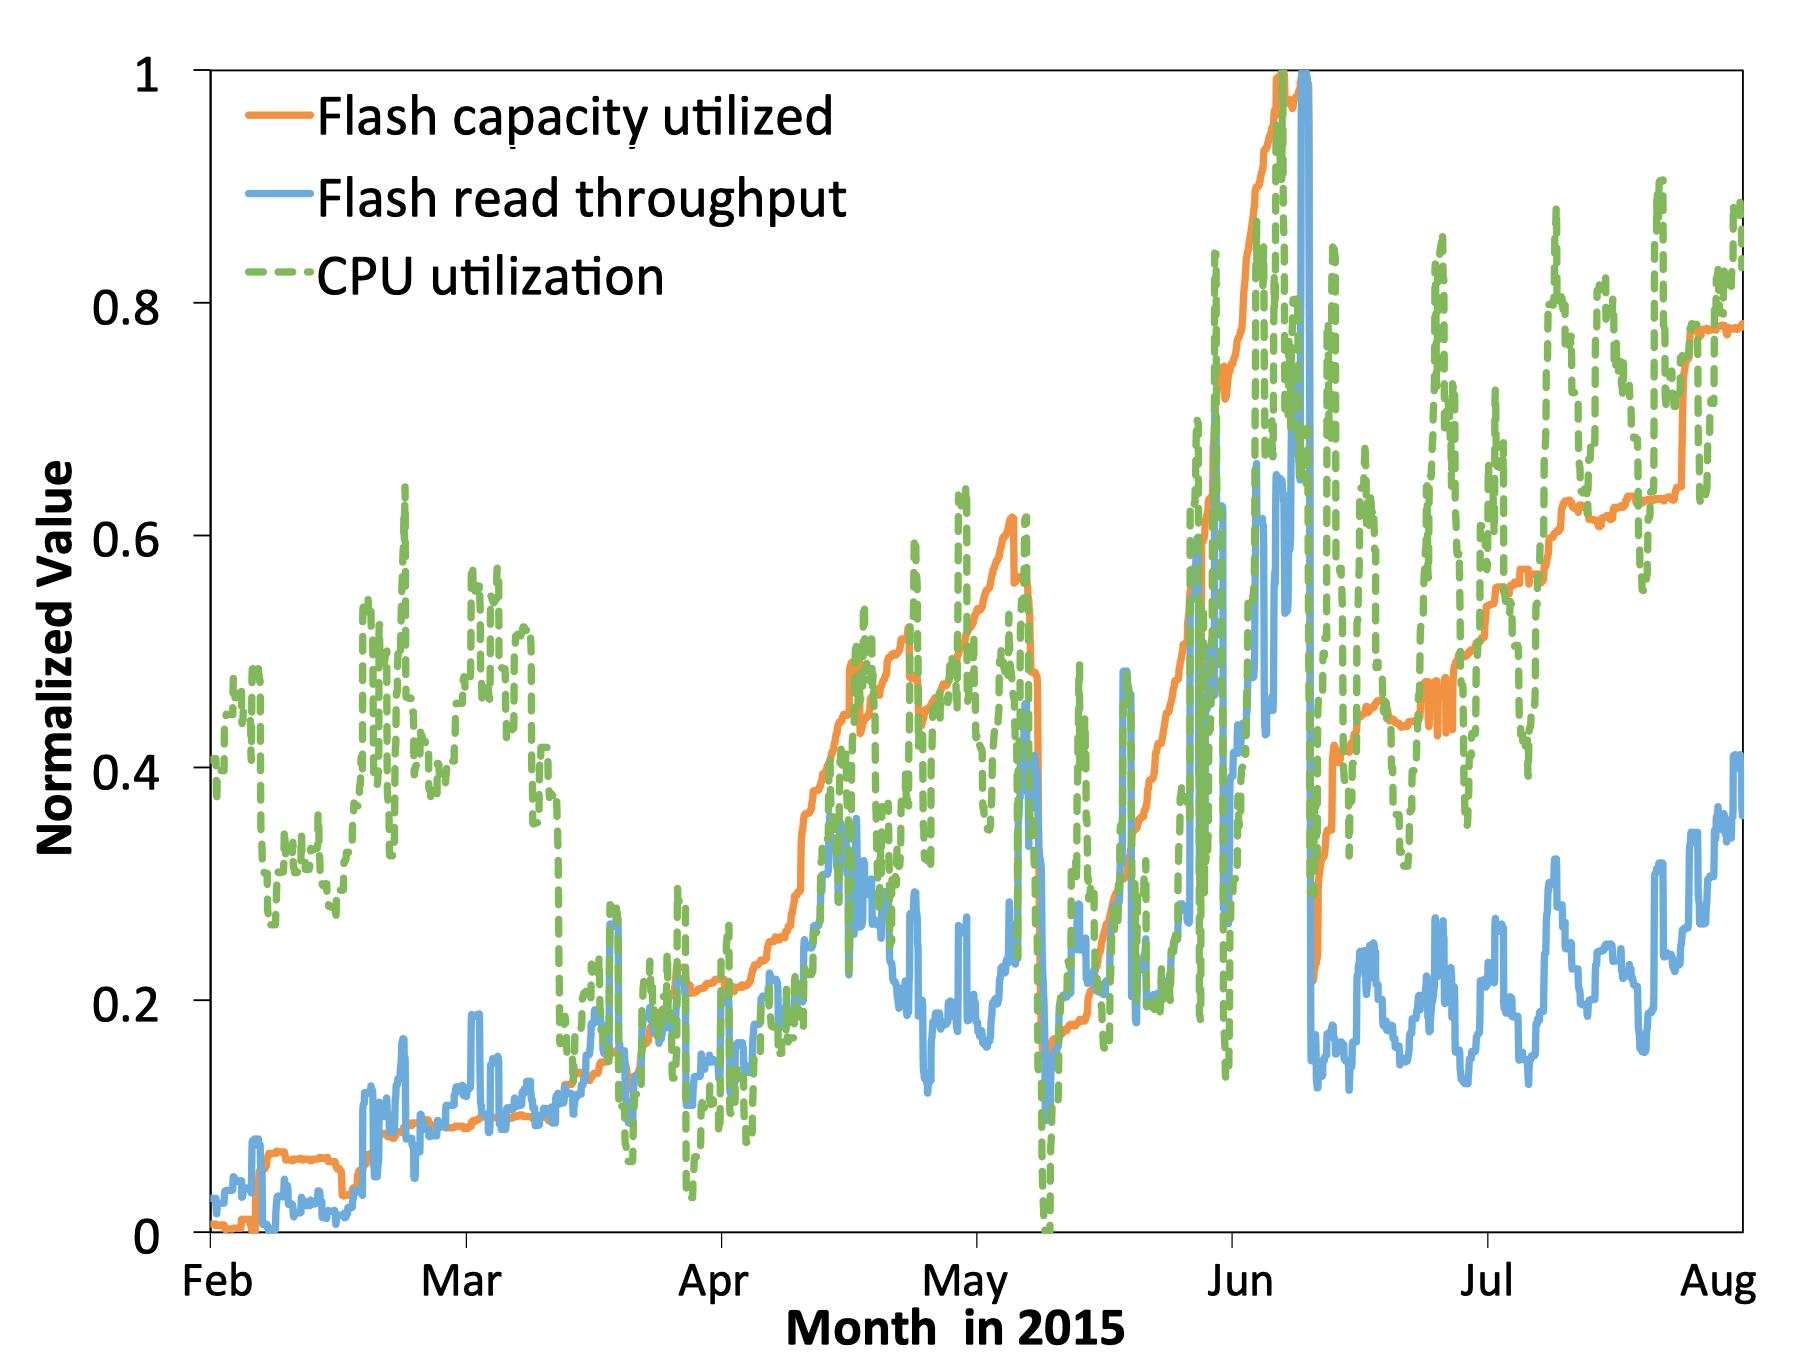
\includegraphics[scale=0.4]{Figures/storage/facebook_storage_ultilization.png}
\decoRule
\caption{Fackebook的一个机器集群的资源利用情况\cite{klimovic2016flash}。}
\label{fig:facebook_storage_ultilization}
\end{figure}

%----------------------------------------------------------------------------------------
%	SECTION 2
%----------------------------------------------------------------------------------------
\section{相关工作}

\subsection{网络存储}
网络存储是一种特殊的、专用的数据存储服务器。
它有直连式存储(DAS)、网络附加存储(NAS)和存储区域网(SAN)三种架构形式。
通常,网络存储服务器包含了一个小型的服务器和很多存储设备,它可以直接接入网络,不需要应用服务器的干预,用户可以通过网络直接读取存储服务器上的数据。

直连式存储指的是将存储设备通过SCSI接口连接到一台服务器使用。
网络附加存储是一种带有小型服务器的存储设备,这个服务器上装配有文件系统,这样的存储设备可以直接接入到普通的网络。
存储区域网是指专门为存储搭建的一个独立的网络,专门同于存储通信。

网络存储将数据集中管理,将存储负载从应用服务器上解耦出来,降低了应用服务器的运营成本,也在一定程度上解决了存储容量不足的问题。
但这种技术也存在着各种各样的问题。
直连式存储仍然存在着存储资源不能在服务器间动态分配的问题。
网络附加存储使用普通的网络,其性能受网络影响大。
存储区域网的缺点是造价昂贵、成本过高。

\subsection{分布式文件系统}
分布式文件系统通过网络将多台机器的存储设备组织起来,通过文件系统的形式来管理和使用这些存储设备,并向用户提供同一的操作接口。
著名的分布式文件系统有Google文件系统\cite{gfs}、Hadoop\cite{shvachko2010hadoop}文件系统等等。

分布式文件系统解决了单台服务器的存储容量不足的问题,并向用户提供了方便的操作接口,在底层甚至还提供了容错处理以及一致性保证。
但也存在着延迟高、读写性能差的问题。
而且它对数据的管理力度过大,很多分布式文件系统的使用场景都是大文件,对于小文件的支持不是很好。
并不是所有应用程序都会去使用分布式文件系统,分布式文件系统不能去管理所有已使用和未使用的存储空间,从这个角度来说,它并没有从根本上解决资源使用不均衡的问题。

\subsection{存储资源分离}
存储资源分离指的是将存储资源从计算节点分离出来,应用程序可以任意地访问本地和远端的存储资源。
像Petal\cite{lee1996petal}、Parallax\cite{warfield2005parallax}、Blizzard\cite{mickens2014blizzard}这类系统,
通过实现了一个虚拟的、分布式的磁盘块仓库将多台机器的存储设备整合,来供文件系统使用,整个过程对应用程序透明,同时还有着很好的性能以及提供容错处理。

存储资源分离技术能提供更细粒度的存储资源管理,对应用程序透明,更具有通用性。
既能解决单台服务器上存储资源不足的问题,也可以解决多台服务器上存储资源使用不足的问题。

%----------------------------------------------------------------------------------------
%	SECTION 3
%----------------------------------------------------------------------------------------

\section{案例分析:闪存资源分离}

\subsection{架构概述}

图~\ref{fig:direct_flash_architecture}展示了传统的闪存使用架构。
每台服务器连着直接连着一块闪存设备,而应用程序只能访问到这块直连的闪存设备。

图~\ref{fig:disaggreagte_flash_architecture}是分离式闪存的架构。
闪存设备在物理上和数据存储层(DataStore Tier)中直接解耦,分成数据存储层和闪存层。
在闪存层增加一个设备服务器,用于接收和处理对闪存设备的读写请求。
闪存层还有一个协调管理器(coordination manager),负责选择合理的存储资源,以达到提高闪存资源利用率的目的。
因此在这种架构中,出现了数据存储服务器和闪存设备服务器两种类型的服务器。
数据存储服务器管理和使用CPU和内存,并跟闪存设备服务器通信,发送对闪存设备的读写请求。
通过这种方法,闪存设备和计算节点解耦了,无论闪存服务器是位于本地还是远端,数据存储服务器能够访问任意地去访问。

\begin{figure}
\centering
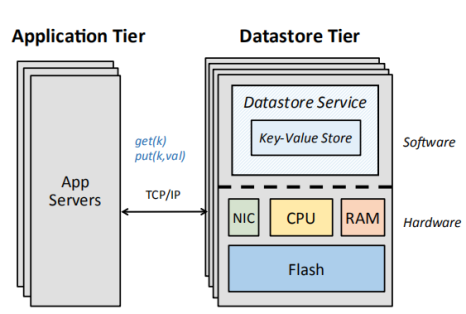
\includegraphics[scale=0.8]{Figures/storage/direct_flash_architecture.jpg}
\decoRule
\caption{直连式闪存架构。}
\label{fig:direct_flash_architecture}
\end{figure}

\begin{figure}
\centering
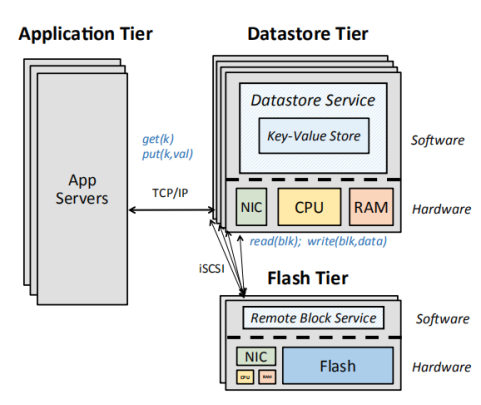
\includegraphics[scale=0.8]{Figures/storage/disaggreagte_flash_architecture.jpg}
\decoRule
\caption{分离式闪存架构。}
\label{fig:disaggreagte_flash_architecture}
\end{figure}

\subsection{设计与实现}

对于本地的闪存设备,数据存储层依然是通过SCSI来访问。
对于远端的闪存设备,数据存储层通过iSCSI(internet small computer system interface)来访问,因为iSCSI能够将对闪存设备的读写操作请求通过网络包的形式发送。
下面我们来介绍对远端闪存设备读操作和写操作的详细流程。

\subsubsection{读操作流程}
iSCSI的initiator接收到来自闪存层的包后,将使用DMA(Direct Memory Access)技术将包的数据从NIC模块转移至内核内存。
内核解析获取的包,拆离出数据内容,将之放在iSCSI的PDU。iSCSI层将PDU数据复制到SCSI缓存。
此时应用就可以从SCSI缓存中直接获取数据。

\subsubsection{写操作流程}
iSCSI层的initiator能控制传输数据的时间,数据存储层维护一个指向协议数据单元(Protocol Data Unit, PDU)的指针。
iSCSI层对要写的数据进行包装(加入信息头等),然后由内核将PDU传输给闪存层。
其中包括的NIC和SCSI的缓存读写则取决与TCP/IP栈的实现。

\subsection{性能评估}

\subsubsection{延迟分析}
数据存储层使用RocksDB键值存储,利用mutilate负载生成器\cite{leverich2014mutilate}生成大量用户进程,进行大量的查询操作,
营造期望的每秒查询率(Queries Per Second, QPS)。图~\ref{fig:read_latency_CDF}展示了在无负载系统下,
本地闪存与远程闪存读取数据的用户延迟的累积分布函数(Cumulative Distribution Function)。
远程闪存的用户延迟显然高于本地闪存,在曲线的95\%处,远程闪存读取延迟约比本地闪存高260微秒。
由于延迟SLA在5到10毫秒左右,远远高于微秒数量级,所以远程闪存的延迟代价在可接受范围内。

\begin{figure}
\centering
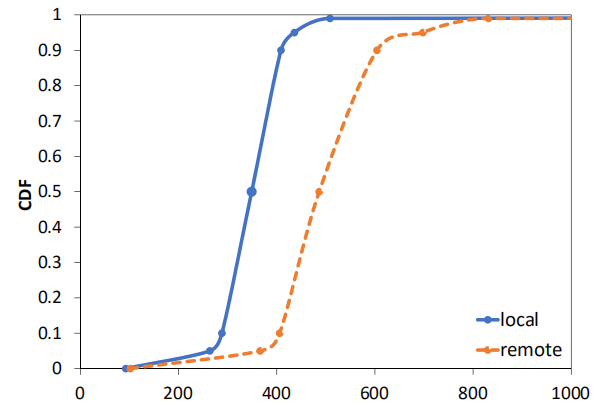
\includegraphics[scale=0.8]{Figures/storage/read_latency_CDF.jpg}
\decoRule
\caption{读操作延迟的CDF曲线。}
\label{fig:read_latency_CDF}
\end{figure}

\subsubsection{吞吐量分析}
为测试本地闪存和远程闪存的吞吐量指标,控制应用层的每秒请求率(QPS),并描绘点(QPS,延迟),图~\ref{fig:QPS_latency}展示其吞吐量性能。
由图分析,在相同延迟情况下,远程闪存吞吐量约为本地闪存的80\%。表观上,远程闪存的吞吐量受到了较严重的影响。
一方面,这是存储设备性能和资源利用率等的权衡,远程闪存的理念是牺牲了部分性能,换取更好的资源利用率。
另一方面,可以通过扩展数据存储层的CPU来补偿这些吞吐量损失。

\begin{figure}
\centering
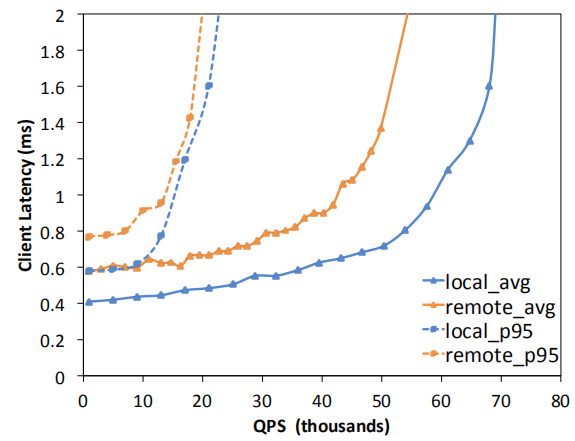
\includegraphics[scale=0.8]{Figures/storage/QPS_latency.jpg}
\decoRule
\caption{单SSDB服务器的延迟-QPS曲线。}
\label{fig:QPS_latency}
\end{figure}

\subsubsection{敏感度分析}
通过在SSDB中增加循环进程,创造不同CPU负载的环境,测试远程闪存的QPS对不同参数的曲线变化率(敏感度)。
图~\ref{fig:QPS_CPUintensity}展示了本地闪存和远程闪存在不同CPU负载下的QPS。二者在CPU负载较低的环境下,本地闪存较远程闪存有更高的QPS,
意味着远程闪存的性能受到一定影响,而在CPU处于较高负载的环境下,本地闪存与远程闪存的QPS相差无几,
意味着此时主要瓶颈不在iSCSI通讯上。同时,本地闪存的QPS受CPU负载大小的影响比远程闪存大,也就是说,远程闪存的性能表现更加稳定。

图~\ref{fig:QPS_percentage}展示了在相同请求数量下,本地闪存和远程闪存的QPS随写请求占总请求的比例变化曲线。
二者的QPS都随着写请求比例增加而增加,因为写操作的返回是异步的,其效率比读操作高。
二者的QPS差值在不同的写操作比例下差别不大,可以得出结论,读写操作所占比例对本地闪存和远程闪存性能差距影响不大。

\begin{figure}
\centering
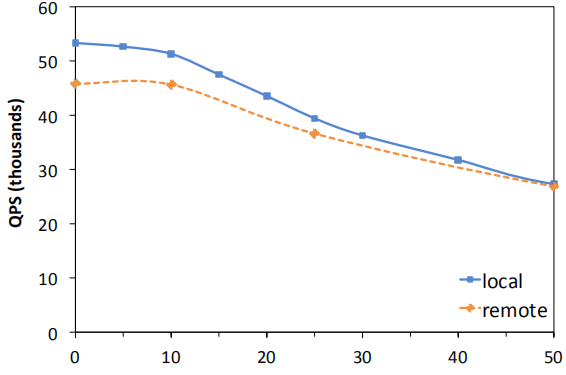
\includegraphics[scale=0.8]{Figures/storage/QPS_CPUintensity.jpg}
\decoRule
\caption{QPS随CPU负载变化曲线}
\label{fig:QPS_CPUintensity}
\end{figure}

\begin{figure}
\centering
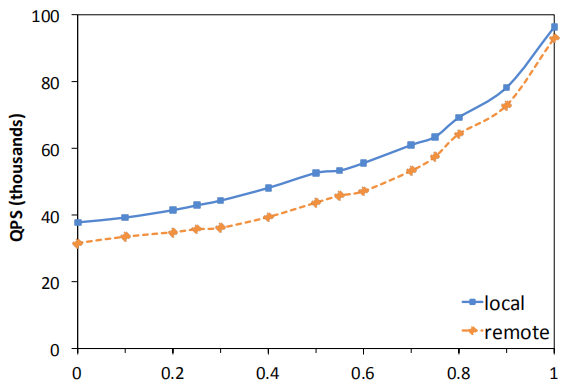
\includegraphics[scale=0.8]{Figures/storage/QPS_percentage.jpg}
\decoRule
\caption{QPS随读操作占比变化曲线。}
\label{fig:QPS_percentage}
\end{figure}

\subsubsection{多服务端性能分析}
实际情况中,机群中服务器主机与闪存时多对多的关系,所以分析多服务端共享同闪存集群的性能很有实际价值。
图~\ref{fig:2SSDB_latency_QPS}和图~\ref{fig:3SSDB_latency_QPS}分别展示两个SSDB服务器主机和三个SSDB服务器主机时,本地闪存与远程闪存的延迟-QPS曲线图。
毫无疑问,本地闪存的QPS性能始终比远程闪存更高。值得一提的是,三个SSDB环境相较于两个SSDB环境下,远程闪存的QPS性能损失代价更严重。

\begin{figure}
\centering
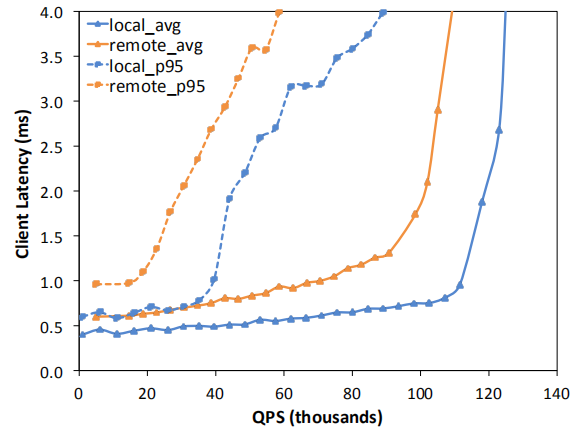
\includegraphics[scale=0.8]{Figures/storage/2SSDB_latency_QPS.jpg}
\decoRule
\caption{2个SSDB服务共享闪存下,延迟-QPS曲线。}
\label{fig:2SSDB_latency_QPS}
\end{figure}

\begin{figure}
\centering
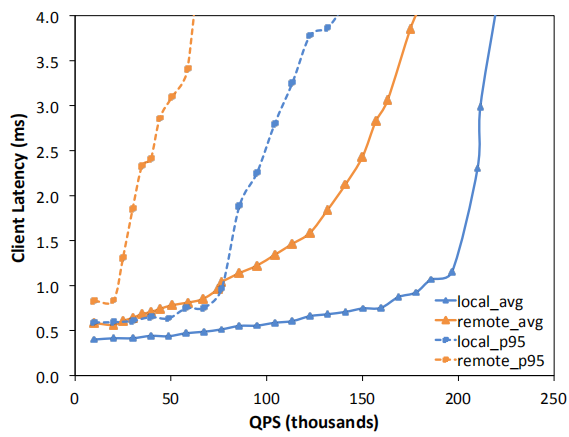
\includegraphics[scale=0.8]{Figures/storage/3SSDB_latency_QPS.jpg}
\decoRule
\caption{3个SSDB服务共享闪存下,延迟-QPS曲线。}
\label{fig:3SSDB_latency_QPS}
\end{figure}

\subsection{存储分离适用情境分析}
通过计算直连式闪存(Direct-attached flash)和远程闪存(disaggregation flash)的主要消耗C$_{direct}$和C$_{disagg}$,对存储分离进行优势评估。
直连式闪存的消耗包括闪存读写的消耗和数据存储端CPU、RAM、NIC的消耗两部分,远程闪存则包括闪存读写的消耗,数据存储层CPU、RAM、NIC的消耗和闪存层CPU、RAM、NIC的消耗。
这些消耗的权重为目标数据与实际数据的比值,如目标QPS与实际QPS的比值。
计算而得的消耗越大,意味着其资源利用越差,反之则越好。
引入新的评估指标,消耗节约比例。
消耗节约比例含义为使用远程闪存比直连式闪存节约的消耗比例。
若消耗节约比例值为正,则表示该环境参数下远程闪存消耗比直连式闪存小;反之则远程闪存消耗更大。

图~\ref{fig:compute_storage}展示了在计算强度比例因子和存储空间比例因子分布空间下,相应的消耗节约比例。
由图例的对称性可以分析而得,闪存读写的消耗与数据存储层的CPU、RAM、NIC消耗大致相等。
在不同的情景假设下(对应图中不同的二维坐标),对资源的分配权衡也是不一样的。
若闪存资源的价值比CPU、内存低,那么服务器将倾向高闪存空间和低计算强度,对应图例的右下半边区域,该区域的消耗节约比例大于零,
意味着远程闪存消耗比直连式闪存低,则此情境下,服务器主机更适合于远程闪存。
若闪存资源的价值比CPU、内存高,那么服务器将倾向低闪存空间和高计算强度,对应图例的坐上半边区域,同理,该区域的消耗节约比例大于零,
远程闪存消耗比直连式闪存低,服务器主机更适合于远程闪存。
若闪存资源与CPU、内存资源价值相当,对应图例的对角线区域,该区域的消耗节约比例小于零,
也就是远程闪存消耗比直连式闪存高,此时服务器主机更适合直连式闪存。

\begin{figure}
\centering
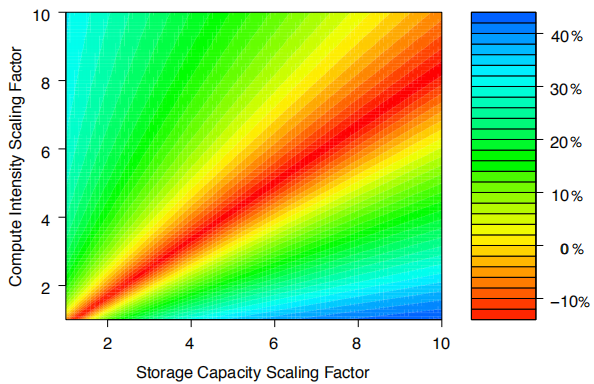
\includegraphics[scale=0.7]{Figures/storage/compute_storage.jpg}
\decoRule
\caption{消耗节约比例-计算强度比例因子-存储空间比例因子分布图}
\label{fig:compute_storage}
\end{figure}

\subsection{案例小结}
Klimovic等人\cite{klimovic2016flash}对闪存分离策略做了充分的研究,分析了闪存分离带来的容量和IO利用率优势,
也客观展示了资源分离带来的性能损失,并提出了弥补性能损失的方法。
在考虑服务器主机整体架构时,不能盲目地强调闪存分离的优势,忽略其带来的性能损失和维护成本。
更加客观的策略是,通过各类资源(如CPU,内存,闪存)的当前价值来定量计算分离式闪存带来的提升及损失孰重孰轻,进而合理取舍。

%----------------------------------------------------------------------------------------
%	SECTION 4
%----------------------------------------------------------------------------------------

\section{本章小结}
本节我们探讨了存储资源的背景,介绍了存储设备和存储技术发展的现状,
并以Klimovic等人\cite{klimovic2016flash}的闪存分离研究工作为切入点,分析了闪存分离的优势及不足,对其作出客观评价。

总结来说,存储资源分离能够实现高程度的存储设备解耦,使得资源管理更加高效便捷,能够大幅提高存储资源利用率,在一定程度上能避免存储资源浪费。
但存储资源分离使得存储框架复杂化,带来额外开发维护成本,且利用网络作为数据传输介质,无疑使得性能也有相当的损耗。
目前大多数解决方案关注点在于架构的设计,力求存储资源分配更加合理化,实际上,减小数据传输带来的性能损耗也是一大研究方向。
利用良好的数据缓存等机制,从根本上减少通过网络传输数据的频率,或许能成为降低性能损耗的良策。
